\documentclass[aps,prc,twocolumn,floatfix,showpacs,a4paper,
nofootinbib,amsmath,amssymb]{revtex4}
%\documentclass[aps,preprint,showpacs,superscriptaddress,
%groupedaddress,amsmath,amssymb]{revtex4}
\usepackage{graphicx}
%\usepackage{dcolumn}
\usepackage{bm}
\usepackage{color}
\usepackage[colorlinks=true, allcolors=blue]{hyperref}
%\usepackage{subfig}
\usepackage{csquotes}
%\usepackage{diagbox}
%\usepackage{lipsum}
%\usepackage{setspace}
\newcommand{\be}{\begin{equation}}
\newcommand{\ee}{\end{equation}}
\newcommand{\ba}{\begin{eqnarray}}
\newcommand{\ea}{\end{eqnarray}}
\newcommand{\bd}{\begin{displaymath}}
\newcommand{\ed}{\end{displaymath}}
\newcommand{\bea}{\begin{eqnarray}}
\newcommand{\eea}{\end{eqnarray}}
\newcommand{\di}{{\rm d}}
\renewcommand{\vec}[1]{\mbox{\boldmath$#1$}}
%\DeclareMathOperator{\Artanh}{Artanh}
%\DeclareMathOperator{\Arsinh}{Arsinh}

\begin{document}

\title{A toy model for simulating $\alpha$ particle emissions in $p+ ^{11}B \rightarrow 3 \alpha$ reactions\linebreak at $K_p\le$10 MeV via Monte Carlo method}

\author{Angel Reina Ramirez, V. Magas}
\smallskip

%\affiliation{
%$^1$Departament de Fisica Quantica i Astrofisica,  
%Universitat\! de\! Barcelona,  Martí i Franquès 1, 08028 Barcelona, Spain\\
%$^2$Institut de Ciències del Cosmos,  
%Universitat\! de\! Barcelona,  Martí i Franquès 1, 08028 Barcelona, Spain\\
%$^3$Institute of Physics and Technology, University of Bergen,
%Allegaten 55, 5007 Bergen, Norway\\
%$^4$Frankfurt Institute for Advanced Studies (FIAS), Ruth-Moufang-Str. 1, 60438, %Frankfurt am Main, Germany\\
%$^5$Wigner Research Centre for Physics (RCP), XII. Konkoly Thege Miklós út 29-33, %Postbox 49, 1121 Budapest, Hungary\\
%$^6$Los Alamos National Laboratory, Los Alamos, 87545 New Mexico, USA
%}

%\acknowledgements

%\begin{abstract}

%\end{abstract}
%\date{\today}
\maketitle
%\tableofcontents
%\pacs{25.75.-q, 24.70.+s, 47.32.Ef}

\section{Model description}

\subsection{ $p+ ^{11}B \rightarrow 3 \alpha$ reaction}
We present a toy model for simulating $\alpha$ particle emissions in $p+ ^{11}B \rightarrow 3 \alpha$ reactions. We simulate this reaction in two steps, as it  is illustrated  in Fig. \ref{Reaction}.

\begin{figure}[h]
	\begin{center}
		\resizebox{0.98\columnwidth}{!}
		{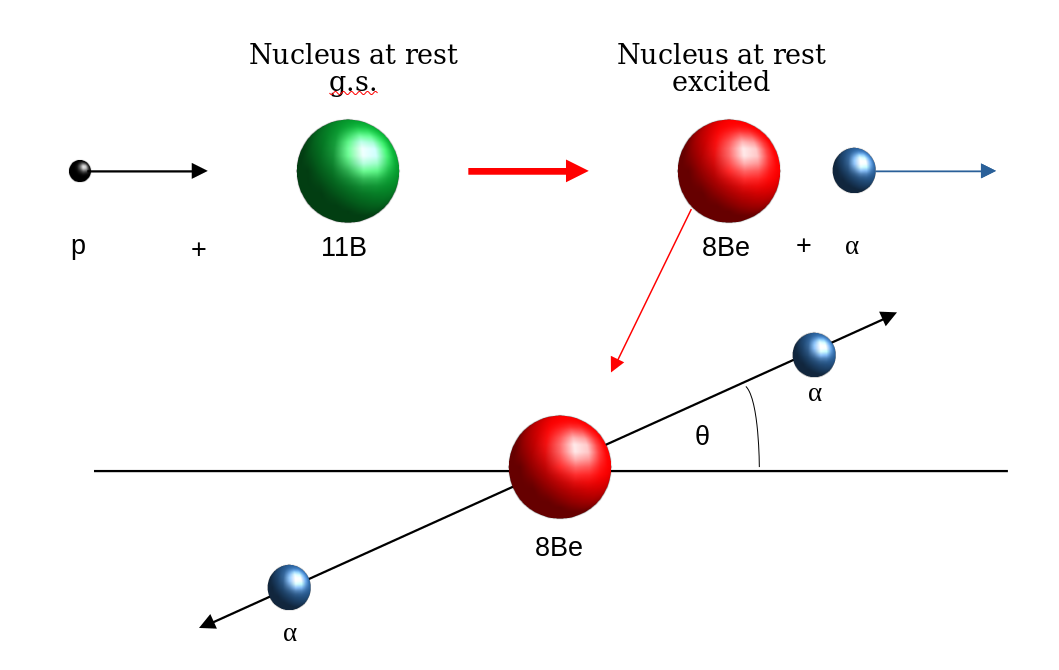
\includegraphics{reaction_scheme.png}}
		\caption{ (color online)
			Reaction scheme.
		}
		\label{Reaction}
	\end{center}
\end{figure} 

In the first step an incident proton with momentum $\vec p_p=(0,0,p_z)$ collides with a $ ^{11}B$ nucleus at rest to produce a $^8Be$ excited nucleus at rest and an $\alpha$ particle moving in the same direction as incident proton. Thus, from the conservation laws, we can obtain: 
\begin{equation}
	\vec p_{\alpha1} = \vec p_p=(0,0,p_z)\,,
	\label{mom1}
\end{equation}
\be
M_p + \frac{p_p^2}{2M_p} + M_{^{11}B} = M_{^8Be}^* + M_{\alpha} + \frac{p_{\alpha1}^2}{2M_{\alpha}}\,.
	\label{ener1}
\ee 
Thus, from Eq. (\ref{mom1}) the polar angle $\theta_1$ at which this first $\alpha$ particle is emitted is constrained to two values: $0$ and $\pi$, depending on if incident proton is moving forward or backward, respectively.

From Eq. (\ref{mom1}) we can find the mass of excited $^8Be$ nucleus
\be
M_{^8Be}^* = M_p + M_{^{11}B} -  M_{\alpha} + \frac{p_p^2}{2M_p}  -  \frac{p_p^2}{2M_{\alpha}}.
\label{ex.mass}
\ee

Later on, in the second step,  $^8Be$ excited nucleus at rest breaks down in two $\alpha$ particles moving in opposite directions. The angles $\theta_2$ and $\theta_3$ at which these two $\alpha$ particles are emitted are randomly generated. Because of momentum conservation law, angle $\theta_3$ is constrained to
\be
\theta_3 = \pi - \theta_2,
\ee
so, actually, we just have to randomly generate $\theta_2$ angle. Similarly, the azimuthal angles are related by the following relation:
\be
\phi_3 = \pi + \phi_2.
\ee
Thus, in spherical coordinates the momentum of emitted $\alpha 2$ and $\alpha 3$ particles are 
\be
\vec{p_{\alpha2}} = p_{\alpha2}\left(sin(\theta_2)cos(\phi_2),sin(\theta_2)sin(\phi_2),cos(\theta_2)\right),
\ee
\be
\vec{p_{\alpha3}} = -p_{\alpha2}\left(sin(\theta_2)cos(\phi_2),sin(\theta_2)sin(\phi_2),cos(\theta_2)\right),
\ee
where $p_{\alpha 2}$ is obtained from the energy conservation law:
\be
p_{\alpha 2}=\sqrt{M_\alpha (M_{^8Be}^* - 2 M_\alpha)}\,.
\label{alpha_for_decay}
\ee

Please note that such a toy models gives maximal possible peaks of the final alpha distribution in the original proton direction: the first alpha always goes in the original proton directions, while the two $\alpha$'s from $^8Be$ decay move in opposite but random direction.

\subsection{Reaction threshold}
Eq. (\ref{ex.mass}) shows that the mass of excited $^8Be$ nucleus, produced in the first step of our reaction, is always bigger that its rest mass. This is because our reaction is exothermic,  $M_p + M_{^{11}B} > M_{\alpha}+M_{^8Be}$, and, thus, from the point of view of the strong interaction our reaction has no threshold and can be activated even by a stopped proton. On the other hand in order to approach a $^{11}B$ nucleus our proton has to overcome the Coulomb barrier, which is 
\begin{equation}
	U_{p+B}=5*\frac{\alpha*\hbar c}{2*R_p+R_{^{11}B}}\simeq 1.61 {\rm MeV},
\end{equation}
where $\alpha$ is the fine-structure constant. Out of this equation we can find the minimal proton momentum which can generate the above reaction: 
\be
p_p^{min}=\sqrt{2 M_p U_{p+B}}\simeq 55.04\ {\rm MeV}.
\label{threshold1}
\ee

\subsection{Proton momentum }
Incident proton is accelerated along the z-axes by an oscillating electric field of frequency $\omega$:
\begin{equation}
E_z = E_0cos(\omega t + \phi)\,,
\end{equation}
what gives an oscillating force acting on protons
\begin{equation}
F_z = e E_0cos(\omega t + \phi) = \frac{dp_z}{dt}\,,
\end{equation}
what finally leads to forced oscillations of the protons. In particular the proton z-momentum oscillates as
\begin{equation}
p_z = \frac{eE_0}{\omega} sin(\omega t + \phi) = p_{z,max} sin(\omega t + \phi)\,,
\label{oscl}
\end{equation}
where its amplitude, $p_{z,max} = \sqrt{2M_pK_p}$, is calculated assuming maximal kinetic energy of  the proton to be $K_p=10$ MeV.   




\begin{figure}[h]
	\begin{center}
		\resizebox{0.98\columnwidth}{!}
		{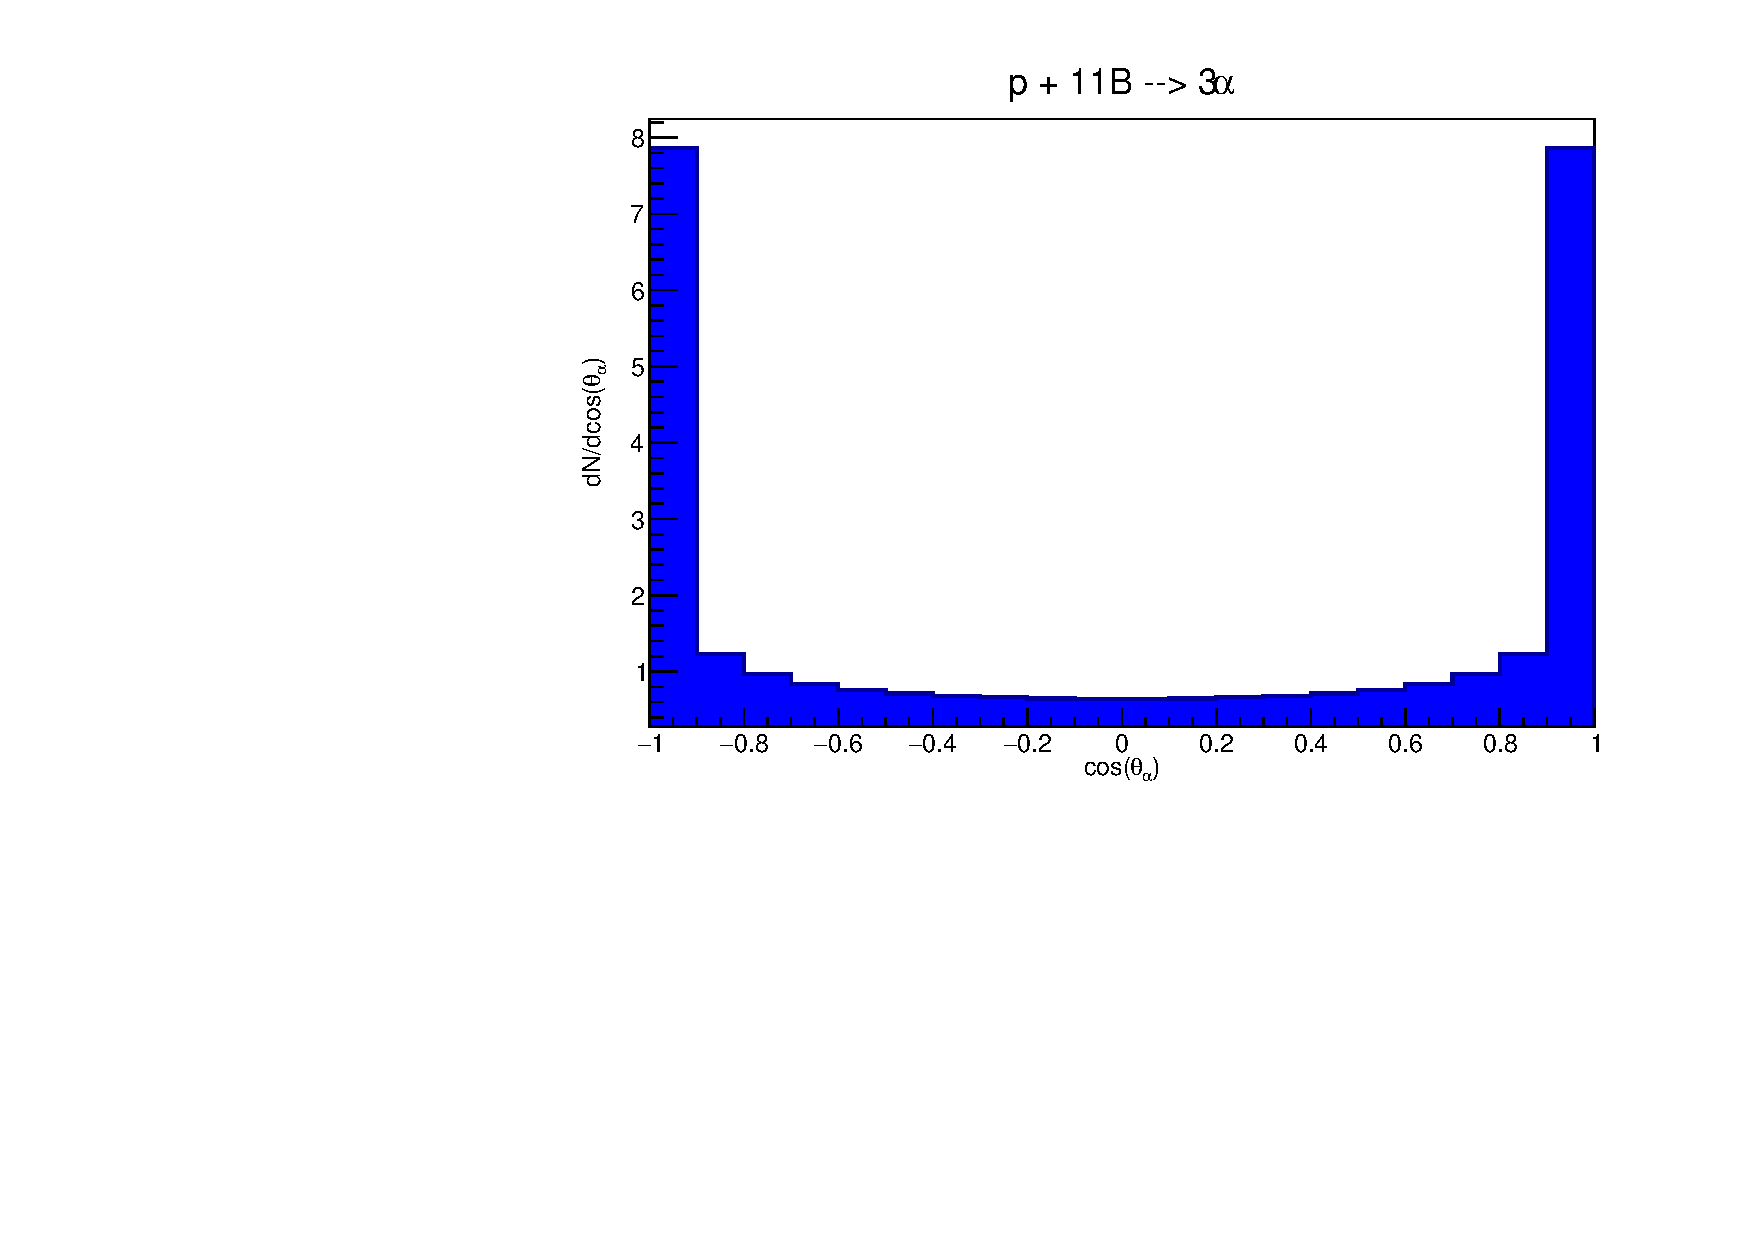
\includegraphics{dNdcostheta.pdf}}
		\caption{ The angular distribution of the produced $\alpha$'s, $dN/d\cos(\theta_\alpha)$. 
		}
		\label{dNdcostheta}
	\end{center}
\end{figure} 

Since the time of the collision is not known and can't be controlled the phase of the proton momentum oscillation is randomly chosen via the pseudorandom number generator: Mersenne twister engine algorithm: 
\begin{equation}
	p_z =\sqrt{2M_pK_p} sin(\phi_p) \,, \quad \phi_p=2\pi*rand\,.
\label{rand}	
\end{equation}



\begin{figure}[h]
	\begin{center}
		\resizebox{0.98\columnwidth}{!}
		{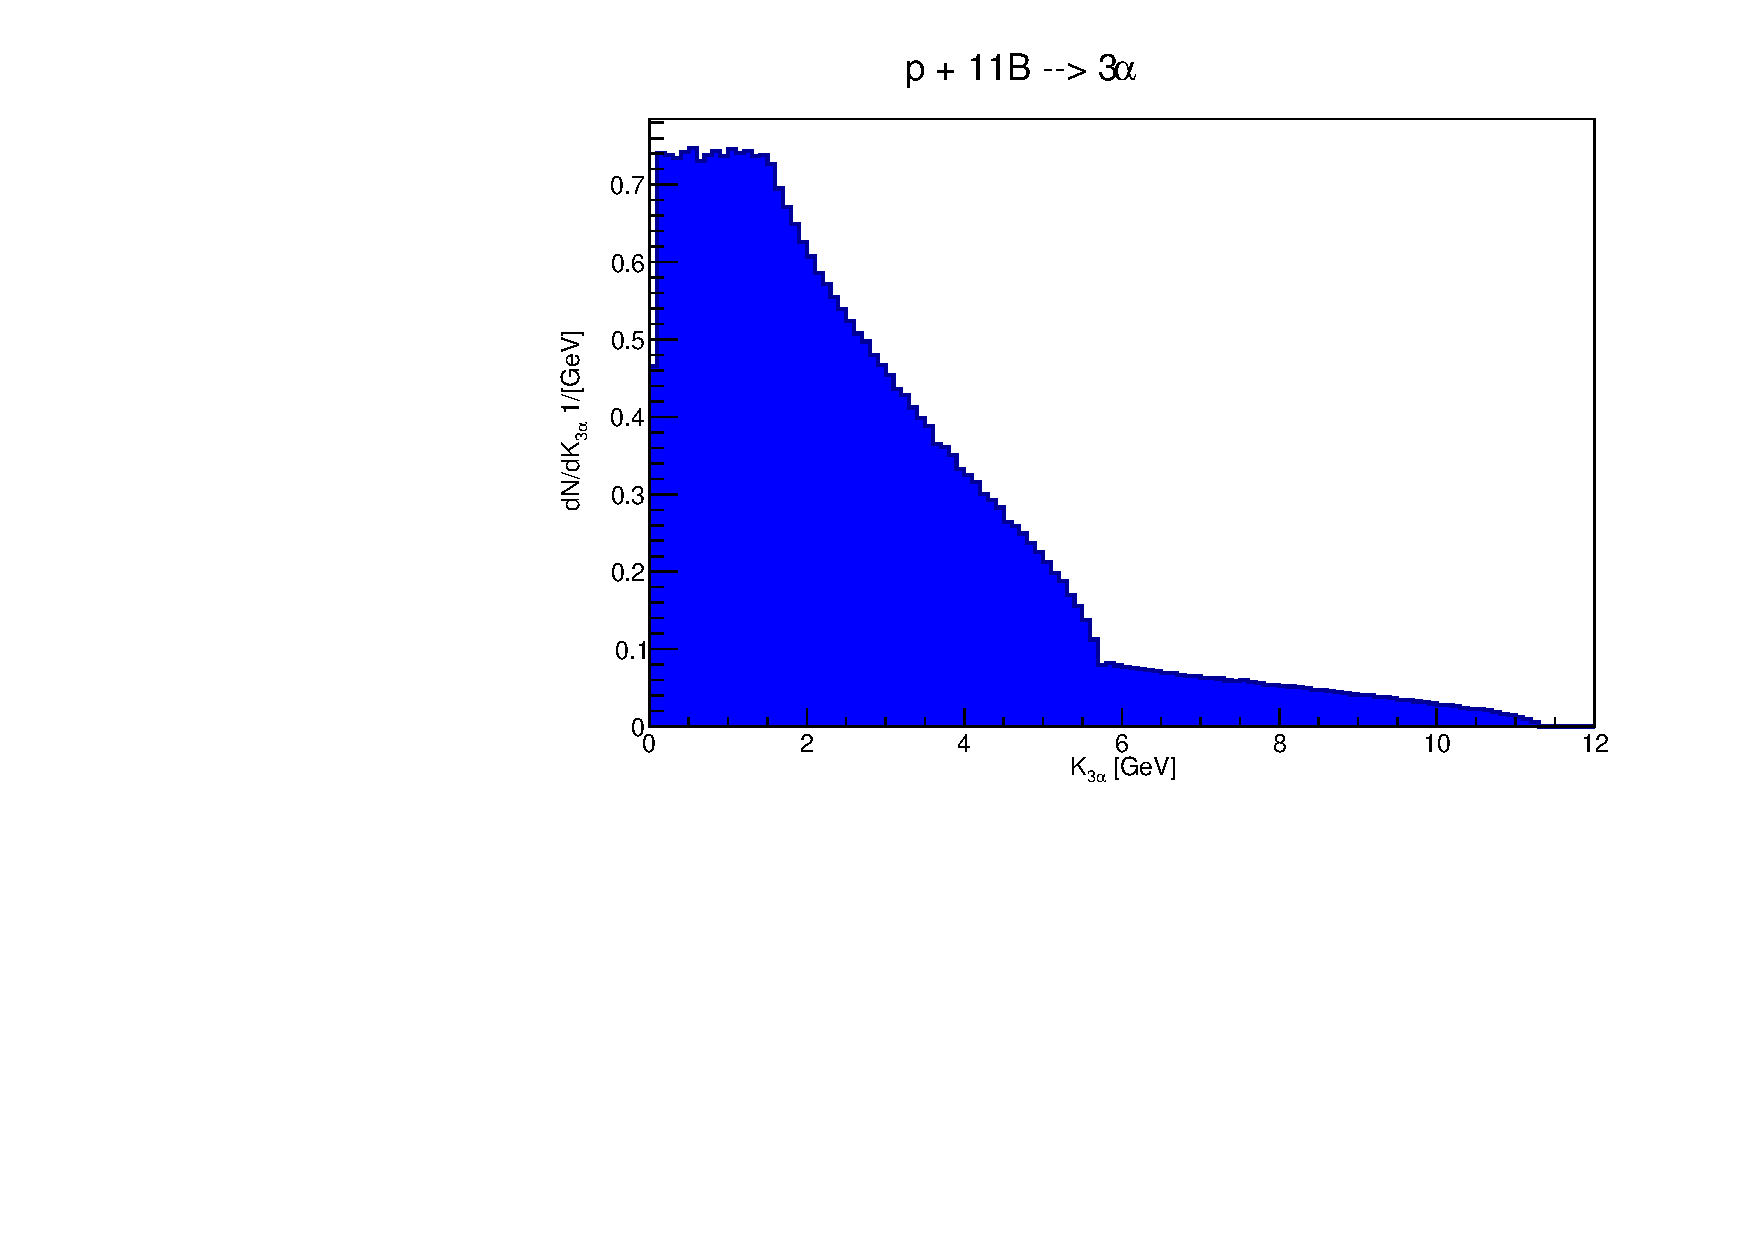
\includegraphics{dNdK.pdf}}
		\caption{ the energy distributions of emitted $\alpha$ particles, $dN/dK_{\alpha}$.
		}
		\label{dNdK}
	\end{center}
\end{figure} 



Please note, that if we generate $p_z < p_p^{min}$ from eq. (\ref{threshold1}) this can not initiate the studied reaction and such an event is just ignored.  


\section{Results}



In this section we present the results of our study, namely the angular distribution of the produced $\alpha$'s, $dN/d\cos\theta_\alpha$,  in Fig. \ref{dNdcostheta},  and the energy distributions of emitted $\alpha$ particles, $dN/dK_{\alpha}$ in Fig. \ref{dNdK}. Since the final $\alpha$'s are indistinguishable at the moment we take into account all of these, although the experimental setup may require to apply some cuts in angles and energy. The calculations were performed for 2000 events.  

As it was mentioned before our description always scatters one alpha in the original proton direction, and thus generates peaks is positive and negative directions of Z-axes, i.e. $\theta=0^o$ and $180^o$, as it is clearly seen in Fig. \ref{dNdcostheta}.   

The two peaks of alpha energy distribution, see Fig. \ref{dNdK}, also have a clear explanation. The form of each of these peaks, peaking at forward energy, has to do with the way we generate initial proton momentum, eq. (\ref{rand}). In this equation we generate randomly the (unknown) phase for the oscillating proton momentum, eq. (\ref{oscl}), and due to properties of $\sin$ function the generated proton momenta will concentrate around max and min values, which both 
correspond to maximal possible kinetic energy $\propto p_p^2$. Consequently we will have more events which correspond to $K_p$ initial proton energy than those which correspond to minimal threshold value $U_{p+B}$.

The first peak in the alpha energy distribution corresponds to the first step of the process, where first alpha get the original proton momentum and thus 25\% of the original proton energy, taking into account the Coulomb threshold $[1.6,10]$ MeV.  

The second peak corresponds to the second step of the process, i.e. to the decay of the excited $^8Be$ nucleus. What happens is that in the $p+B \rightarrow 3 \alpha$ reaction always more than $8$ MeV of energy is released: 
$$
2 E_{\alpha_{2}} = M_p + M_{^{11}B} -  3*M_{\alpha} + \frac{p_p^2}{2M_p}  -  \frac{p_p^2}{2M_{\alpha}}
$$
\be
=8.7\ {\rm MeV} +  \frac{p_p^2}{2M_p}  -  \frac{p_p^2}{2M_{\alpha}}.
\label{alpha2}
\ee
This explains the $4.3$ MeV threshold of the second peak. In general, this is good since it allows us to distinguish $\alpha$'s from the first and second step of the reaction by detecting its energy.       




%\section{References}

%\appendix{Appendix I}

\end{document}
